%!TEX root = ../documentation.tex

\chapter{Benutzeroberfläche}

\section{Beschreibung der Benutzeroberfläche}
\subsection{Appstart}
Nach dem erstmaligen Start der App durch anklicken des App Icons gelangt der Benutzer zur in Abbildung \ref{label:startview} gezeigten Benutzeroberfläche.

\begin{figure}[H]
\centering
	\begin{minipage}{0.4\textwidth} 
	\centering
	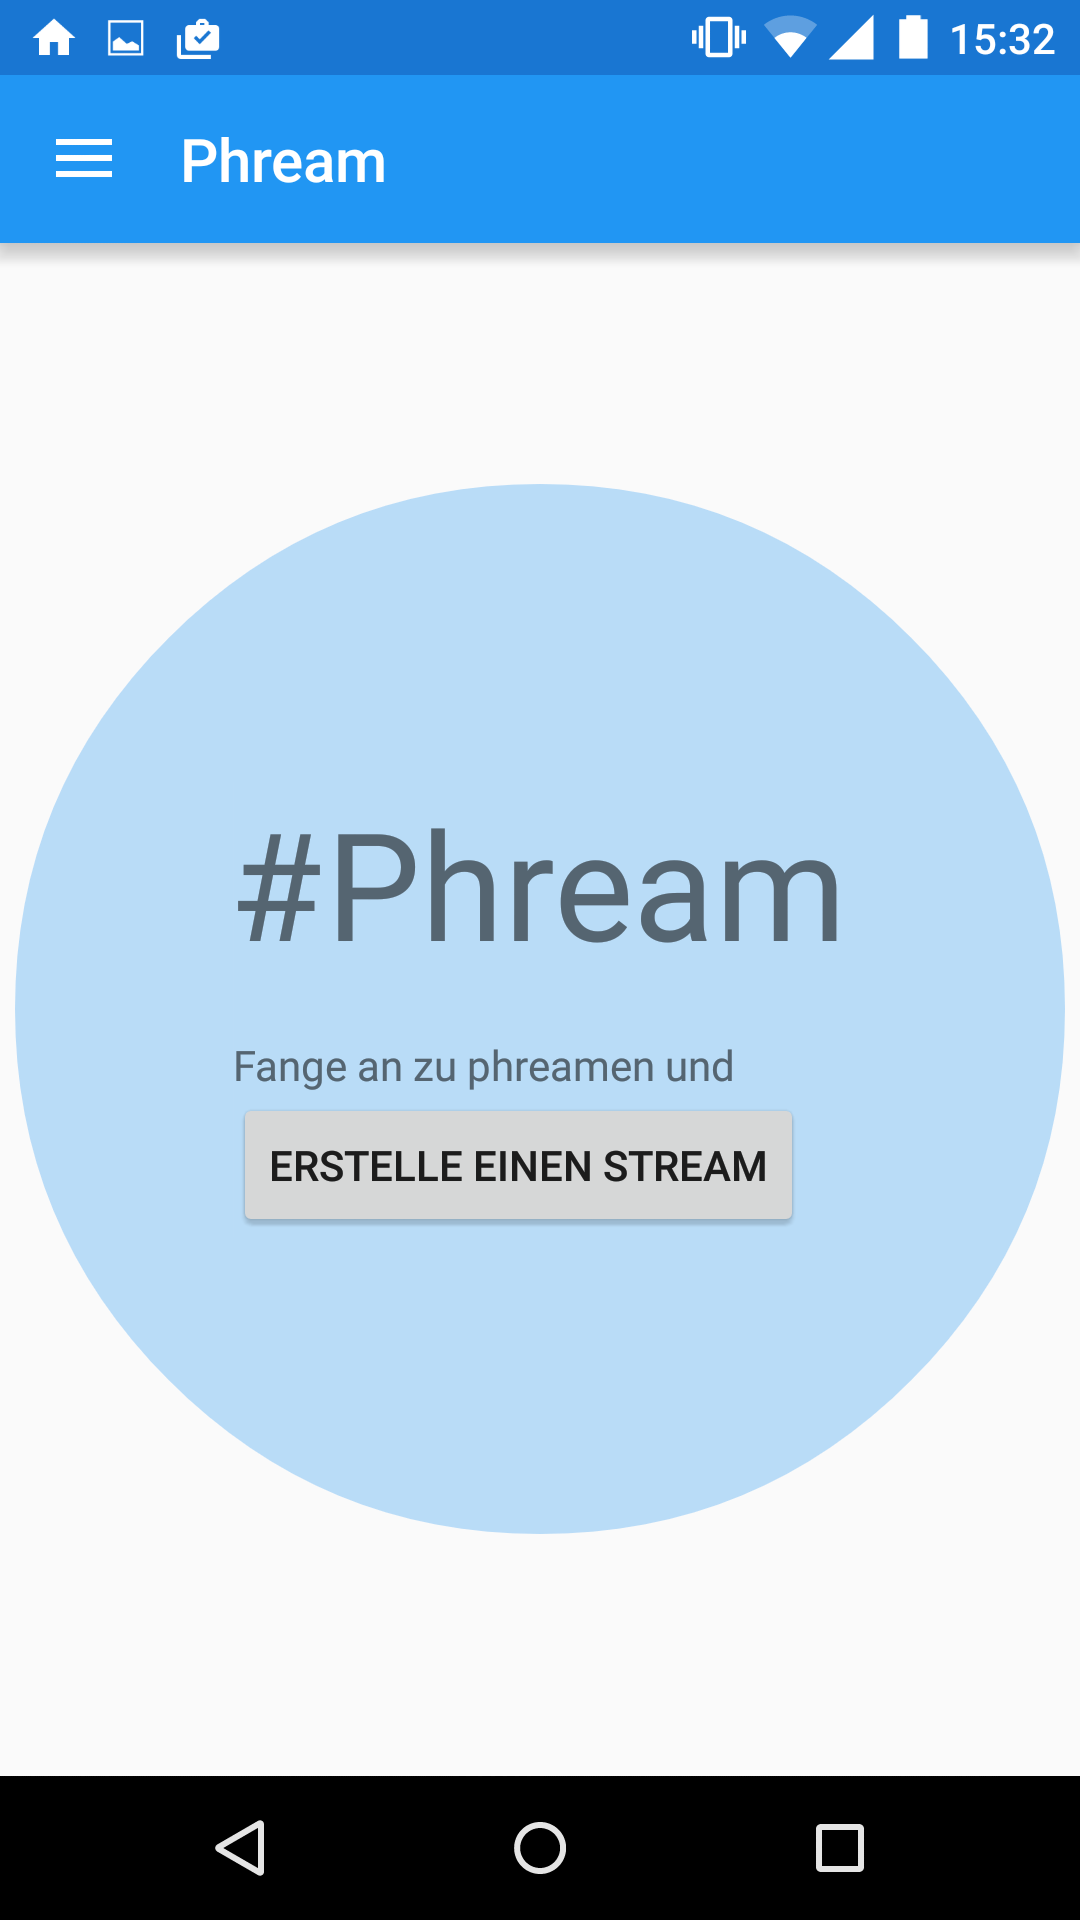
\includegraphics[width=0.6\textwidth]{images/screenshots/startview.png}
	\caption{App-Startansicht}
	\label{label:startview}
	\end{minipage}
	\hfill
	\begin{minipage}{0.4\textwidth}
	\centering
	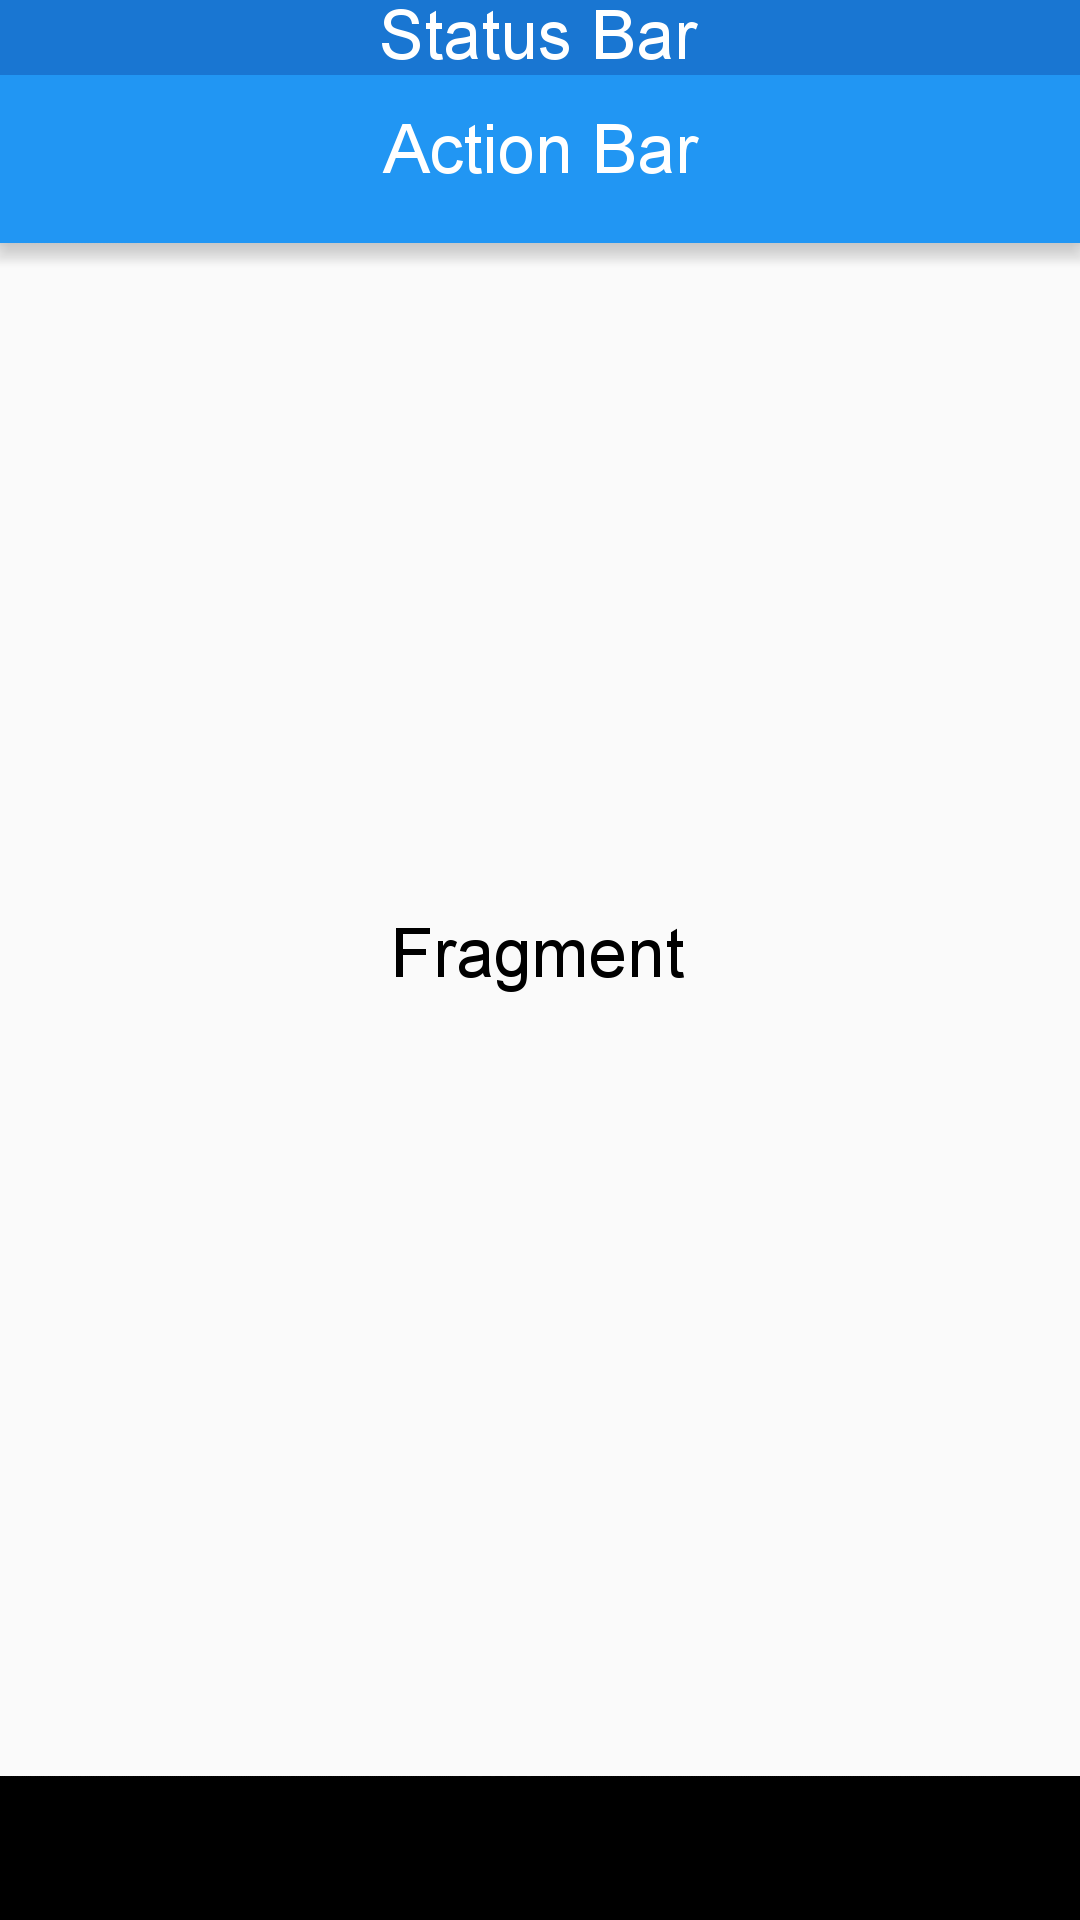
\includegraphics[width=0.6\textwidth]{images/screenshots/startview_schema.png}
	\caption{Schematische Darstellung}
	\label{label:startview_schema}
	\end{minipage}
\end{figure}
Die in Abbildung \ref{label:startview_schema} eingezeichnete Statusbar ist standardmäßig in jeder Ansicht der App zusehen und zeigt allgemeine Statusinformationen zum Androidgerät an. Die Action Bar wird von der App selbst gestaltet und beinhaltet verschiedene Optionen, wie beispielsweise Menüs. Den größten Teil der App nimmt das Fragment in Anspruch. In diesem werden die verschiedenen Informationen der App dargestellt. Das Fragment ist dabei eine Art selbständige \enquote{Sub-Activity}, die einen eigenen Lifecycle, inklusive eigener Action Listener, besitzt.
Das Fragment wird dynamisch durch einen Manager bei Benutzeraktionen ausgetauscht.

In der aktuell angezeigten Startansicht (Abbildung \ref{label:startview}), die beim erstmaligen Start oder wenn Stream (Ordner) angelegt ist, angezeigt wird, beinhaltet das Fragment den dargestellten Text, den Button zum Anlegen eines Streams und den im Hintergrund platzierten Kreis. Durch anklicken des Buttons öffnet sich ein Eingabefenster, in dem ein neuer Streamname eingegeben werden kann. Nach Bestätigung des Streamnamens wird der Stream angelegt und erscheint daraufhin im Navigation Drawer. 

\subsection{Navigation Drawer}

Der Navigation Drawer (Abbildung \ref{label:navigationdrawer}) kann durch klicken auf das Menüicon oben links neben dem Appnamen oder durch einen Swipe vom linken Bildschirmrand geöffnet werden.
In der daraufhin eingeblendeten Ansicht hat der Benutzer die Möglichkeit zwischen verschiedenen Streams zu wechseln und neue Streams anzulegen. Durch anklicken eines Streamnamens wird dieser aktiv und wird daraufhin in der Hauptansicht angezeigt. Durch einen swipe zum linken Bildschirmrand oder durch anklicken des Pfeils links neben dem Appnamen kann der Navigation Drawer geschlossen werden.

\begin{figure}[H]
\centering
	\begin{minipage}{0.4\textwidth} 
	\centering
	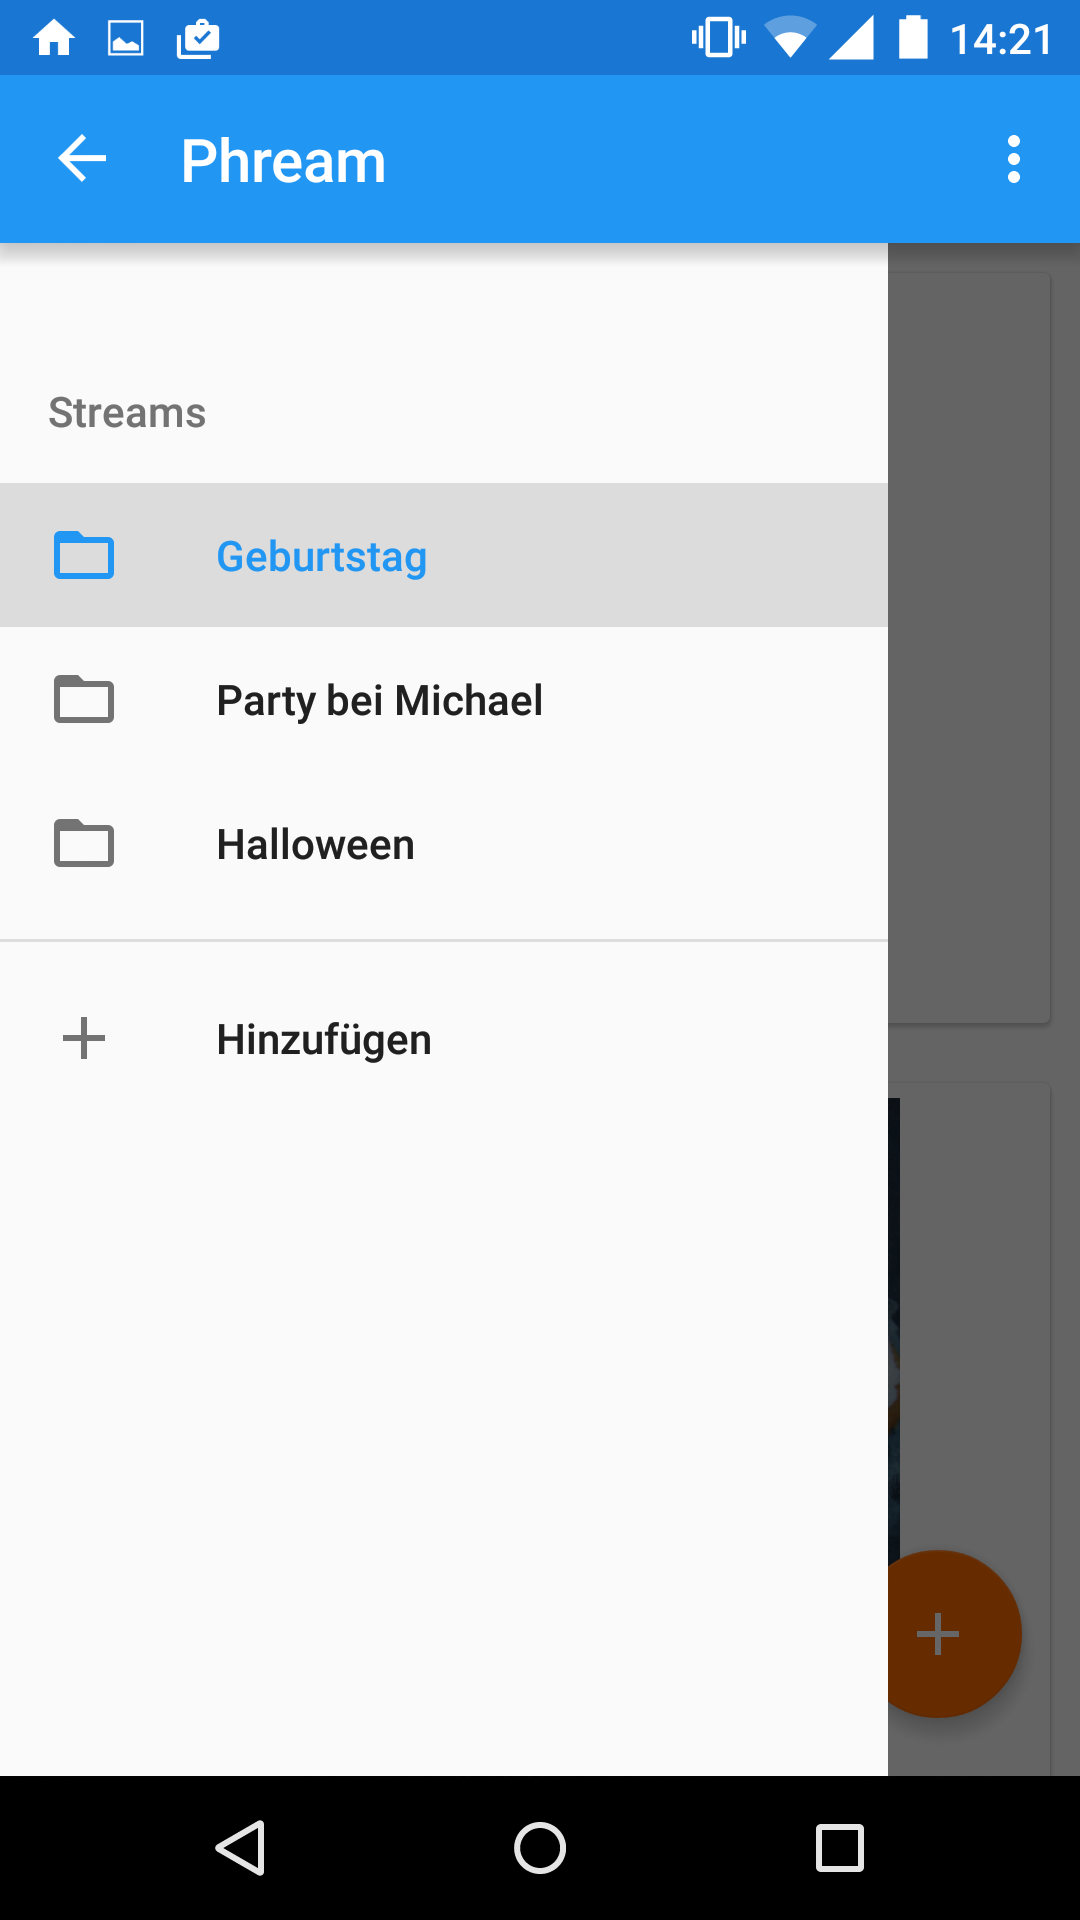
\includegraphics[width=0.6\textwidth]{images/screenshots/navigationdrawer.png}
	\caption{Navigation Drawer}
	\label{label:navigationdrawer}
	\end{minipage}
	\hfill
	\begin{minipage}{0.4\textwidth}
	\centering
	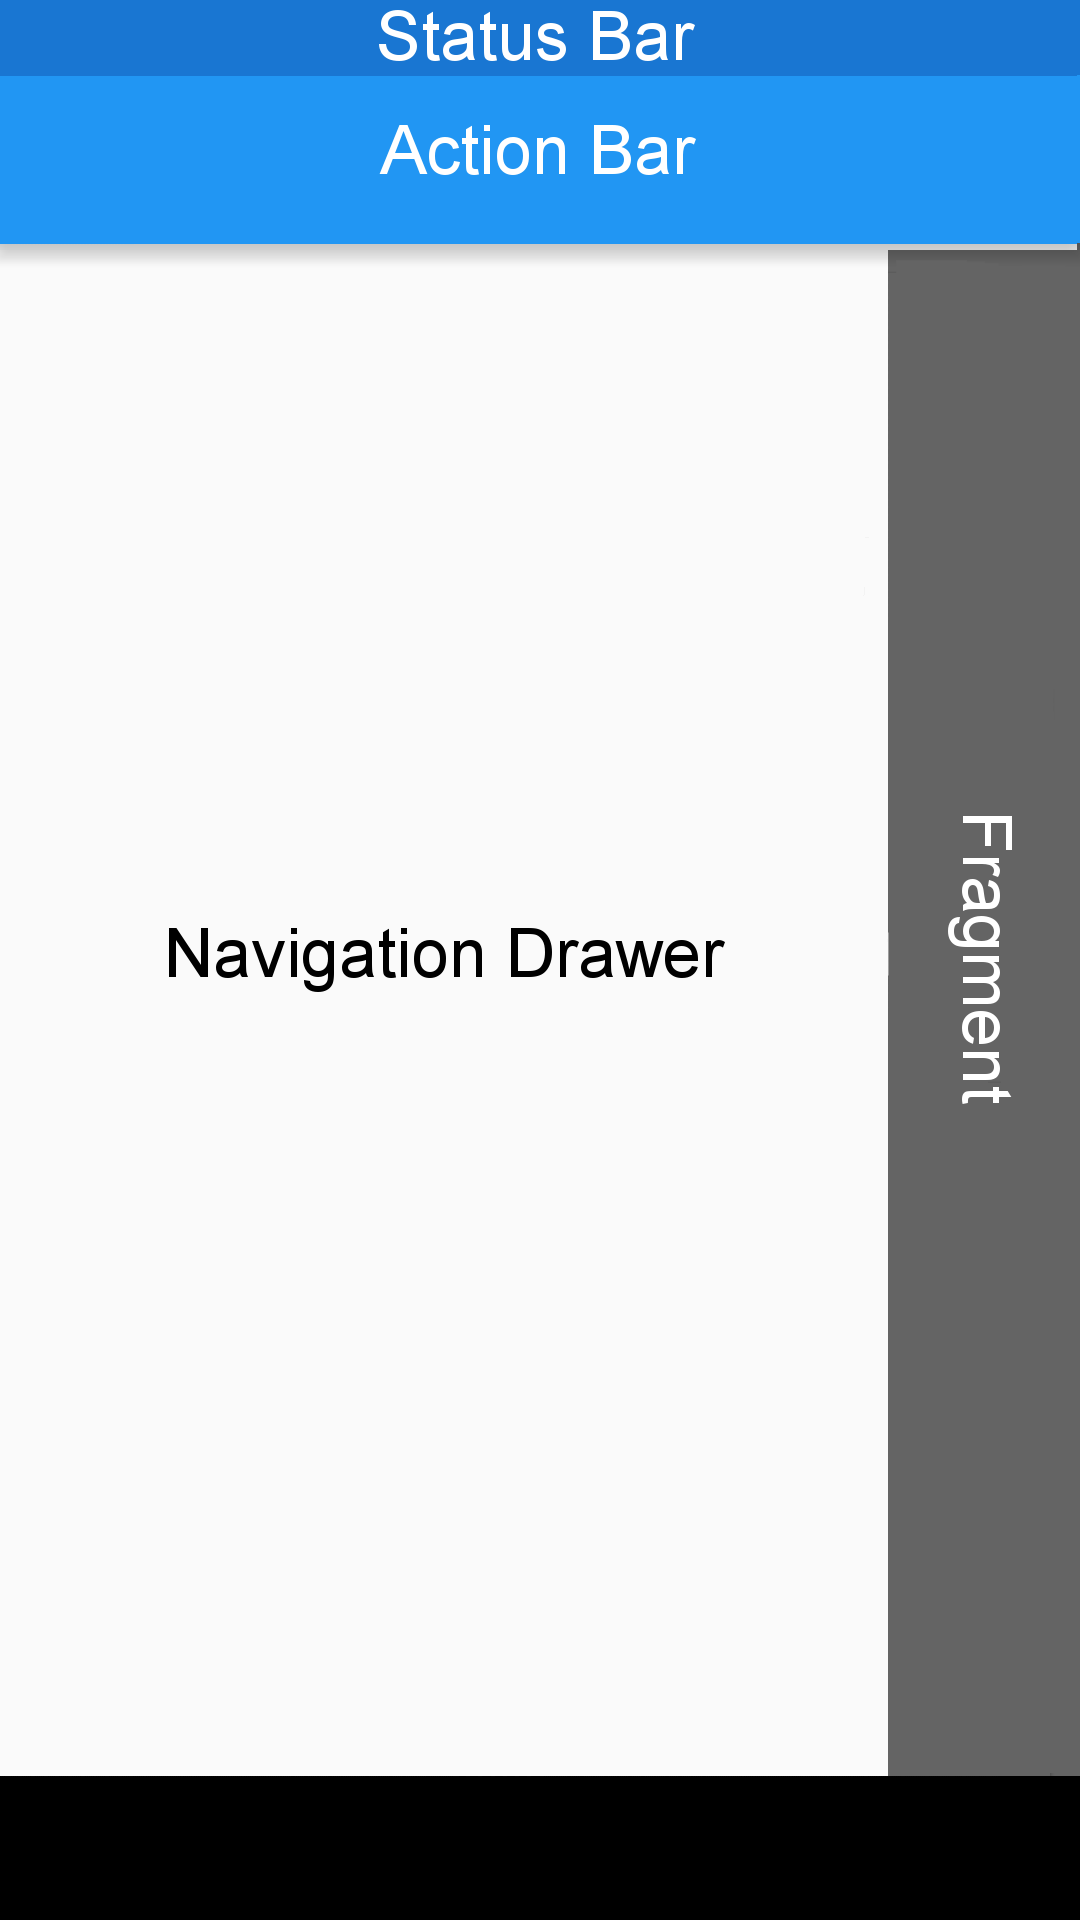
\includegraphics[width=0.6\textwidth]{images/screenshots/navigationdrawer_schema.png}
	\caption{Schematische Darstellung}
	\label{label:navigationdrawer_schema}
	\end{minipage}
\end{figure}
In der schematischen Darstellung (Abbildung \ref{label:navigationdrawer_schema}) ist zu sehen, dass der Navigation Drawer das aktuelle Fragment \enquote{überdeckt} und den restlichen Teil des Fragments abdunkelt. Der Navigation Drawer selbst wird dabei wieder aus einem Fragment zusammengesetzt. In der Action Bar wird dabei der Button zum Öffnen des Navigation Drawer zu einem Pfeil.

\subsection{Streamansicht}
Nach dem Auswählen eines Streams im Navigation Drawer oder beim Appstart (wenn ein Stream angelegt ist) wird dieser in der Hauptansicht angezeigt. Die Streamansicht (Abbildung  \ref{label:streamview}) zeigt alle Bilder an, die dem entsprechenden Stream zugeordnet wurden. Das Fragment wird dabei mit CardViews gefüllt, die eine ImageView mit einem Vorschaubild, dem Bildtitel, sowie Aufnahmeinformationen zum entsprechenden Bild beinhaltet. Der Benutzer kann durch Scroll-Gesten durch die Ansicht navigieren. Das oben rechts in der Action Bar angezeigte \enquote{Options-Symbol} beinhaltet die Optionen, den aktuellen Stream umzubenennen und zu löschen. Beim Löschvorgang eines Streams werden alle Daten zum Stream und dessen Inhalt aus der Datenbank und alle Bilder von der SD-Karte gelöscht.

\begin{figure}[H]
\centering
	\begin{minipage}{0.4\textwidth} 
	\centering
	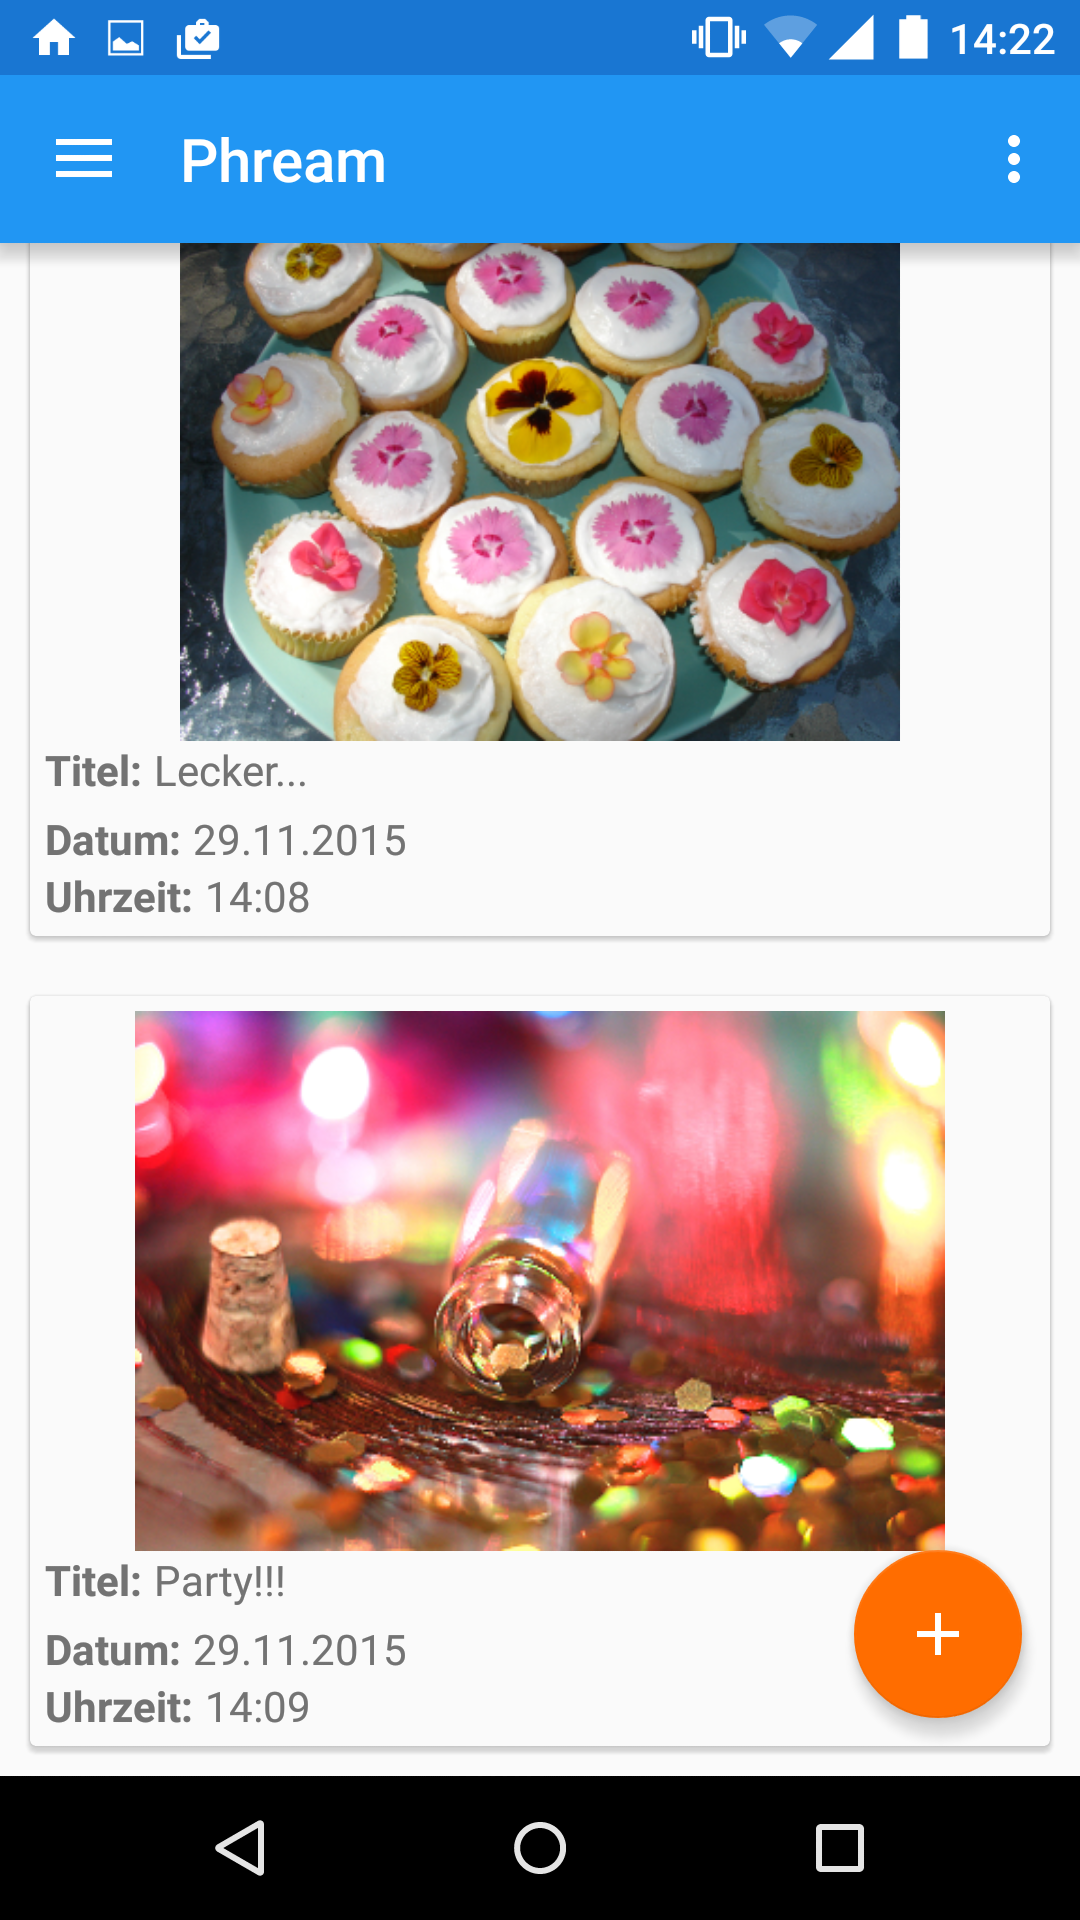
\includegraphics[width=0.6\textwidth]{images/screenshots/streamview.png}
	\caption{Streamansicht}
	\label{label:streamview}
	\end{minipage}
	\hfill
	\begin{minipage}{0.4\textwidth}
	\centering
	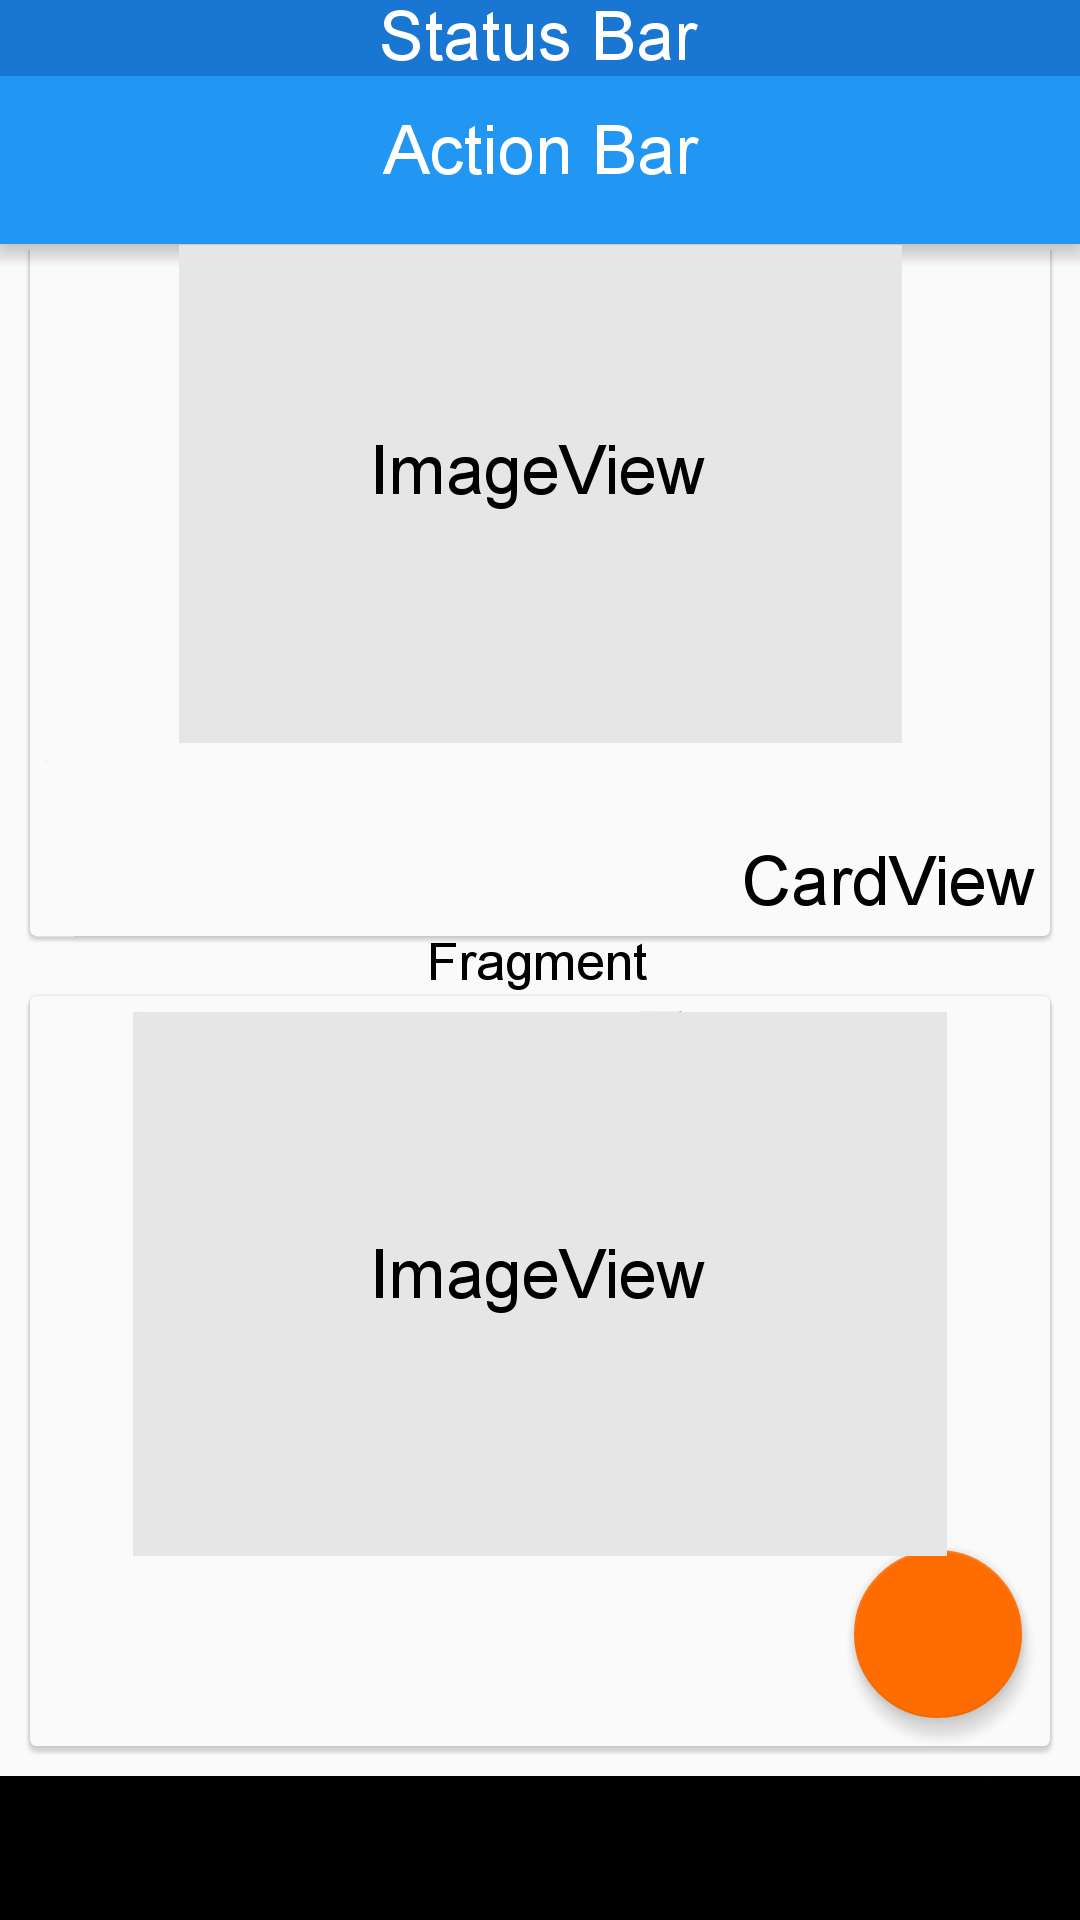
\includegraphics[width=0.6\textwidth]{images/screenshots/streamview_schema.png}
	\caption{Schematische Darstellung}
	\label{label:streamview_schema}
	\end{minipage}
\end{figure}

\subsubsection{Kontextmenü des CardView}

Durch einen \enquote{long tap} auf eine CardView in der Hauptansicht öffnet sich ein Kontextmenü zum aktuellen Bild. Das Kontextmenü bietet verschiedene Optionen, wie das Umbenennen des Bildes, das Löschen des Bildes und einer Export Möglichkeit in die Galerie. Durch antippen der gewünschten Option erscheinen zusätzliche Abfragen je nach Menüeintrag. Es wird beispielsweise beim Umbenennen ein AlertDialog erzeugt, der die Eingabe eines neuen Bildtitels ermöglicht. Beim Löschen oder Exportieren des Bildes sollen eingeblendete AlertDialogs versehentliche Nutzeraktionen abfangen und eine Bestätigung der Aktion vom Benutzer erfragen.

\begin{figure}[H]
	\centering
   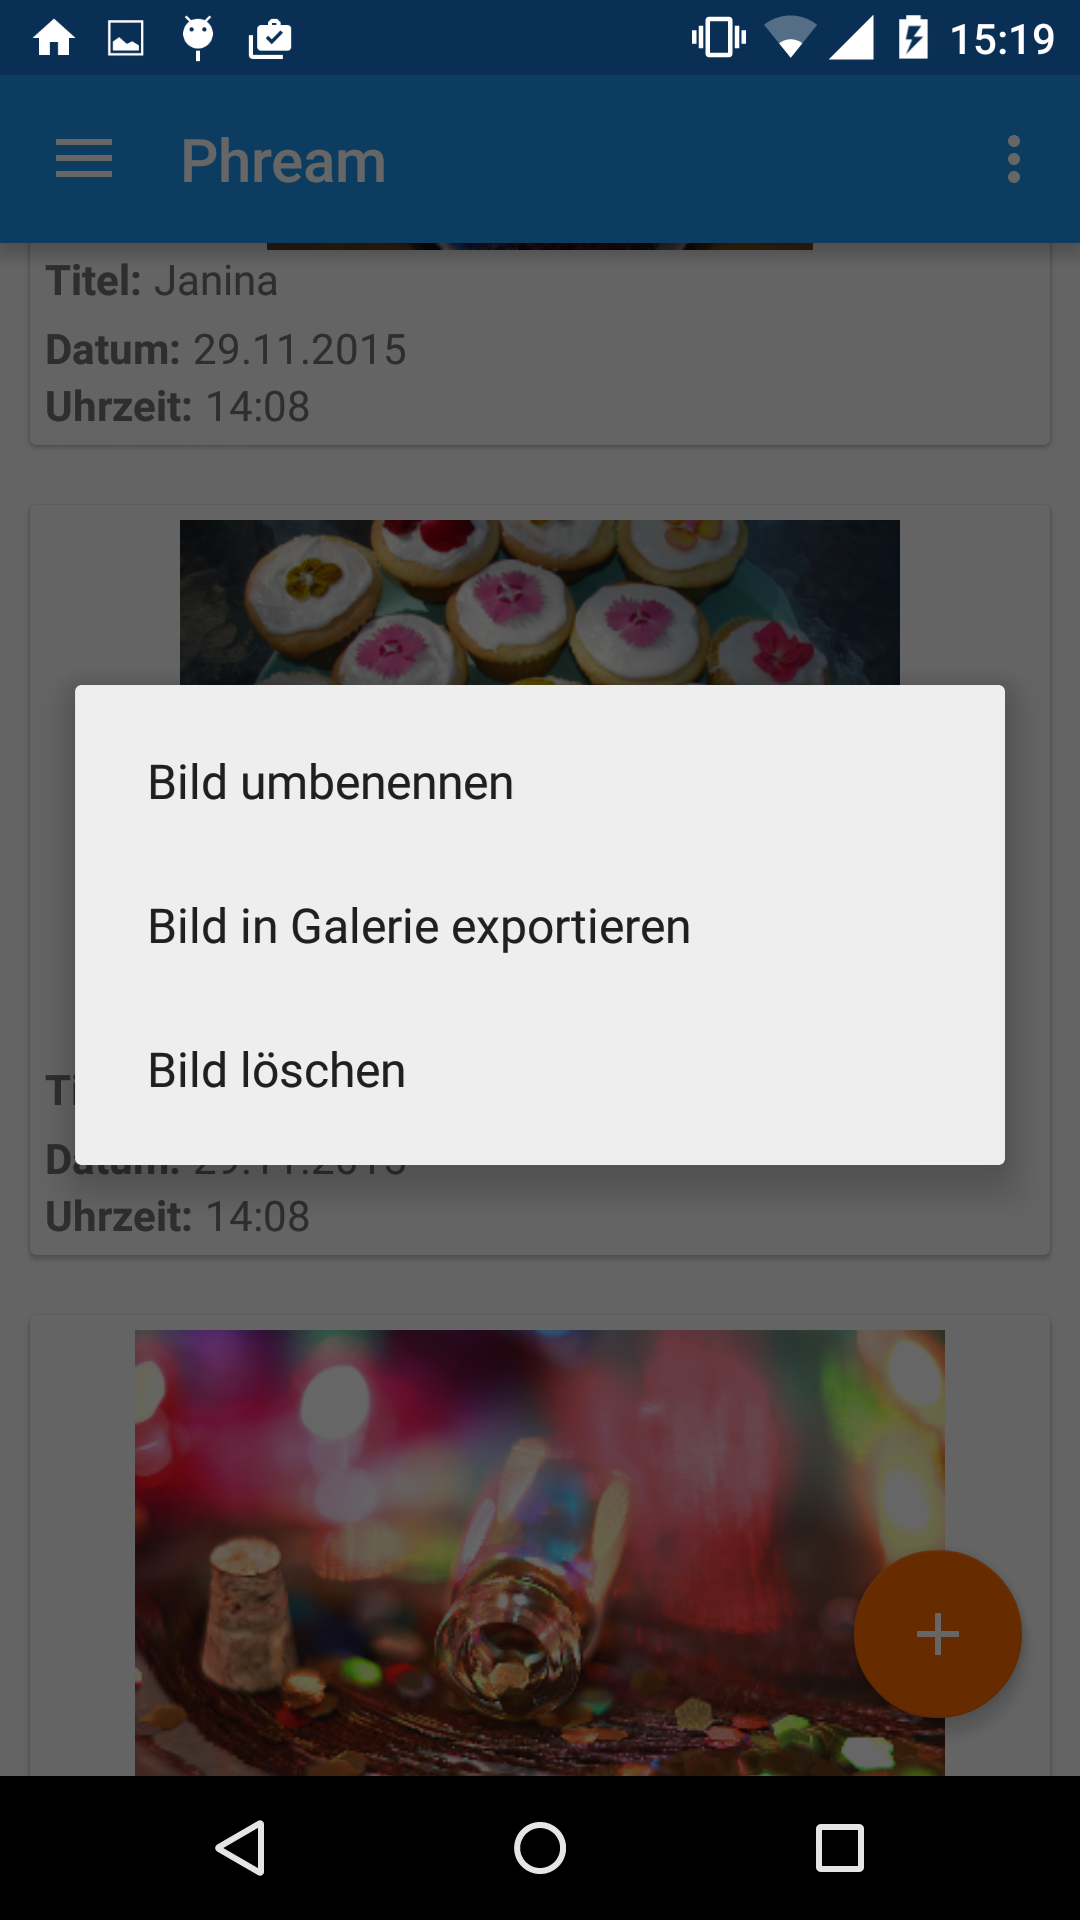
\includegraphics[scale= 0.115]{images/screenshots/contextmenu.png}
  \caption{Kontextmenü - CardView}
\end{figure}

\section{Detailansicht eines Bildes}
Durch anklicken einer Card in der Hauptansicht, öffnet sich eine zweite Activity die eine Detailansicht (Abbildung \ref{label:fullscreenview}) des Bildes im Vollbild ermöglicht. Die Detailansicht besteht dabei aus einer Fullscreenactivity mit einer ImageView, die die gesamte Activity ausfüllt.
\begin{figure}[H]
\centering

\includegraphics[scale=0.09]{images/screenshots/fullscreenview.png}
\caption{Detailansicht eines Bildes}
\label{label:fullscreenview}
\end{figure}

Durch einen \enquote{short tap} wird die Status Bar und die Action Bar wieder eingeblendet und bietet dem Bentuzer verschiedene Interaktionsmöglichkeiten (Abbildung \ref{label:fullscreenview_menu}).

\begin{figure}[H]
\centering
	\begin{minipage}{0.4\textwidth} 
	\centering
	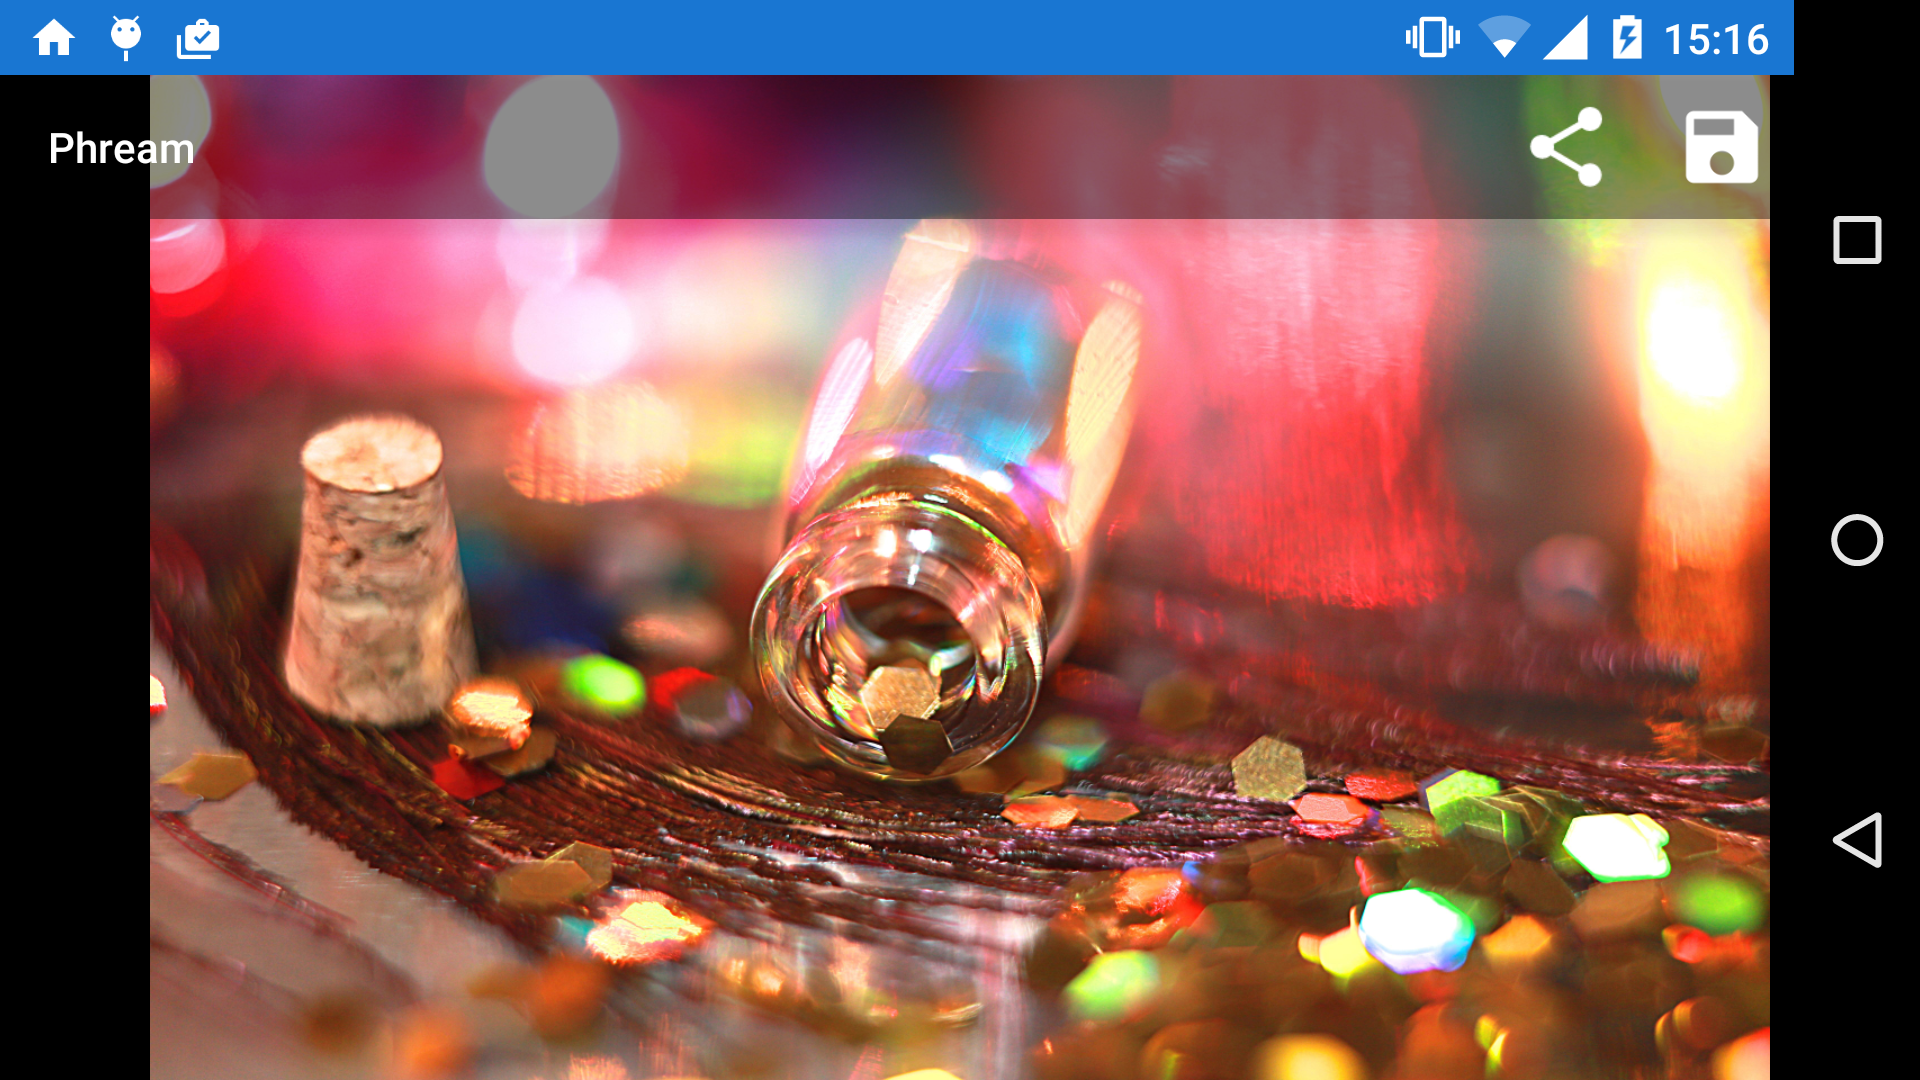
\includegraphics[width=1\textwidth]{images/screenshots/fullscreenview_menu.png}
	\caption{Detailansicht mit Action Bar}
	\label{label:fullscreenview_menu}
	\end{minipage}
	\hfill
	\begin{minipage}{0.4\textwidth}
	\centering
	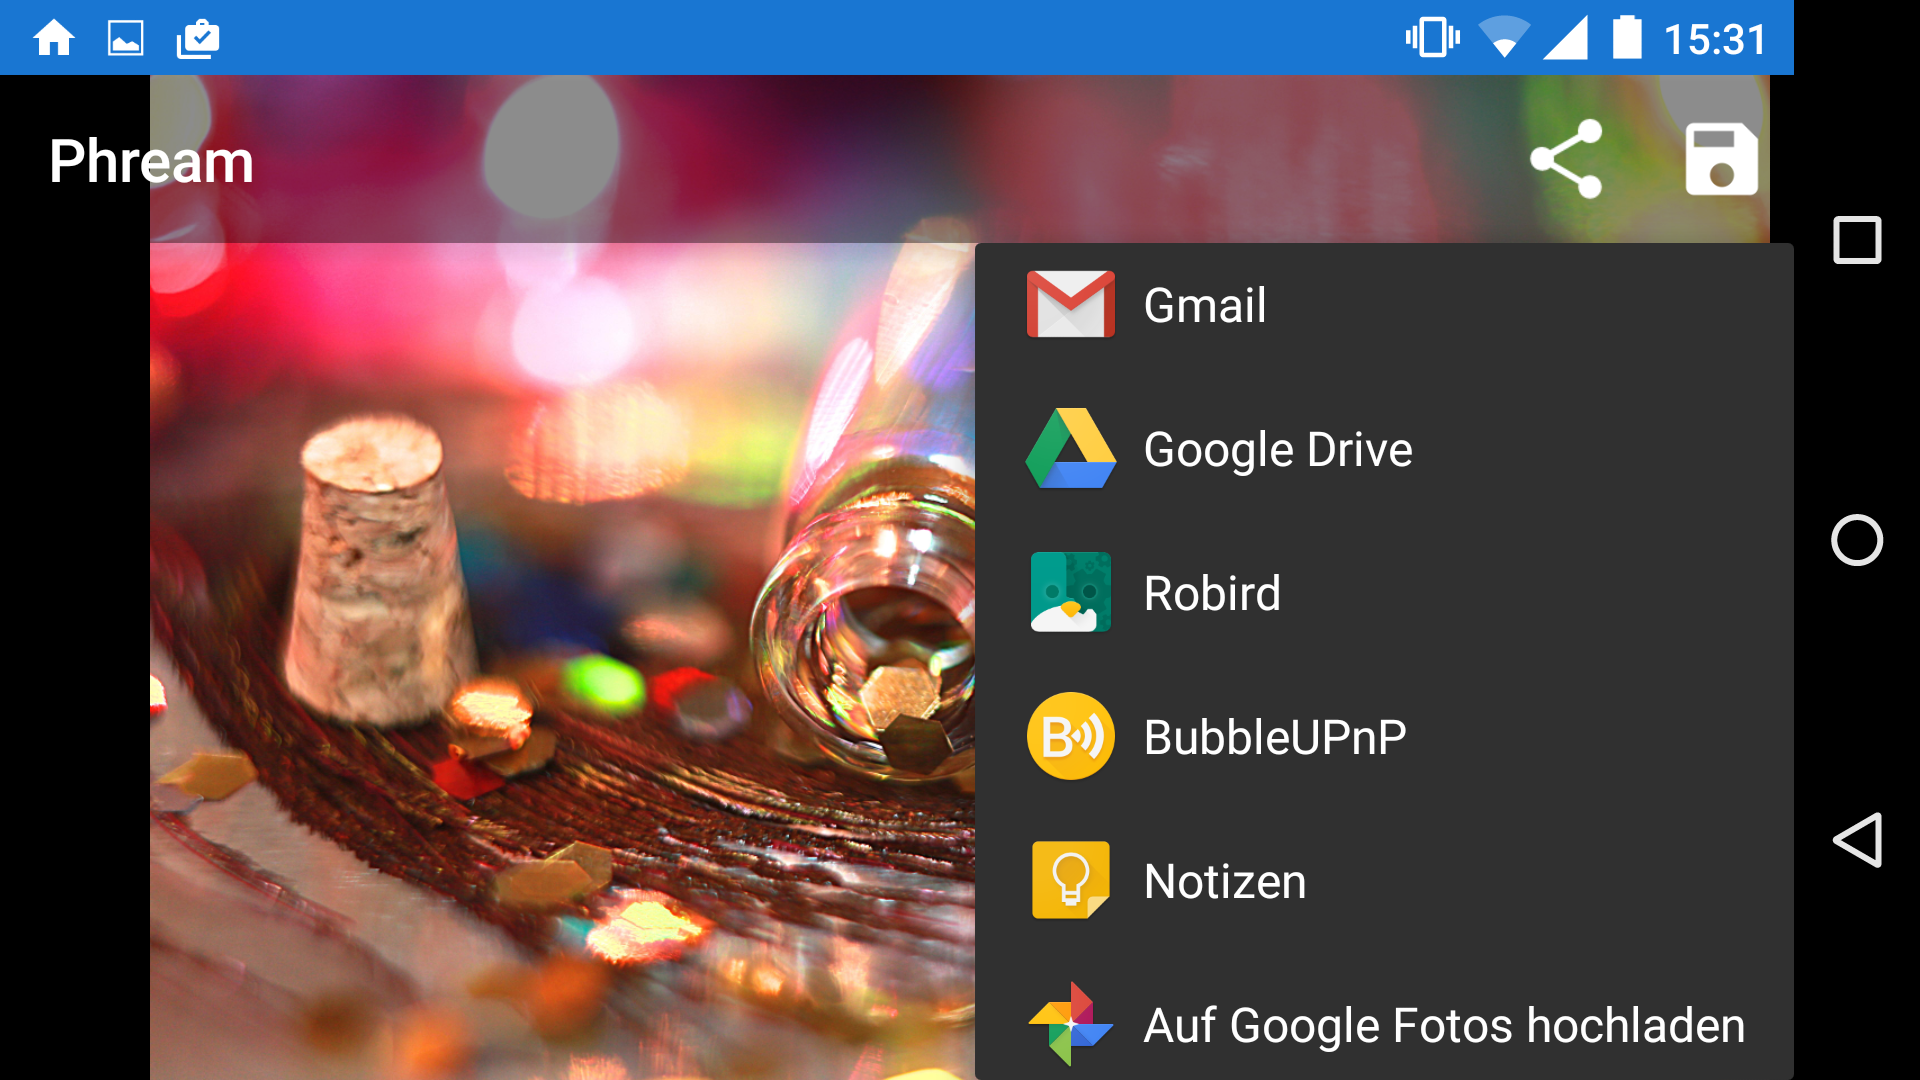
\includegraphics[width=1\textwidth]{images/screenshots/fullscreenview_share.png}
	\caption{Share-Provider}
	\label{label:fullscreenview_share}
	\end{minipage}
\end{figure}

Durch anklicken des \enquote{Speichern-Symbols} oben rechts in der Action Bar kann der Benutzer das aktuelle Bild in die Android Galerie exportieren. Dieses wird daraufhin mit aktuellen Datum und Uhrzeit als erstes in der Android Galerie angezeit. Durch antippen des \enquote{Share-Symbols} öffnet sich der Share Provider (Abbildung \ref{label:fullscreenview_share}) von Android. Der Share-Provider ist eine allgemeines Framework, welches die Option bietet verschiedene Dateien mit anderen Apps zu teilen oder ihnen zur Verfügung zu stellen. Eine Option ist beispielsweise, sofern ein E-Mail Client vorhanden ist, das aktuelle Bild per E-Mail zu versenden.

\section{Der Floating Action Button}
Der Floating Action Button in der Hauptansicht dient der Gruppierung zweier wichtiger Funktionen der App. Dabei bietet der Floating Action Button verschiedene Transformationsverhalten und öffnet durch antippen ein Floating Action Menu mit weiteren Optionen (Abbildung \ref{label:floatingaction_menu}). Weiterhin ist der Floating Action Button leicht durch eine Daumengeste erreichbar und gruppiert die Hauptfunktionalitäten der aktuellen Activity in einem Punkt. Je nach angetippten Menüeintrag startet der Galerieimport oder ein Kamera-Intent zum Aufnehmen eines Fotos.

\begin{figure}[H]
\centering
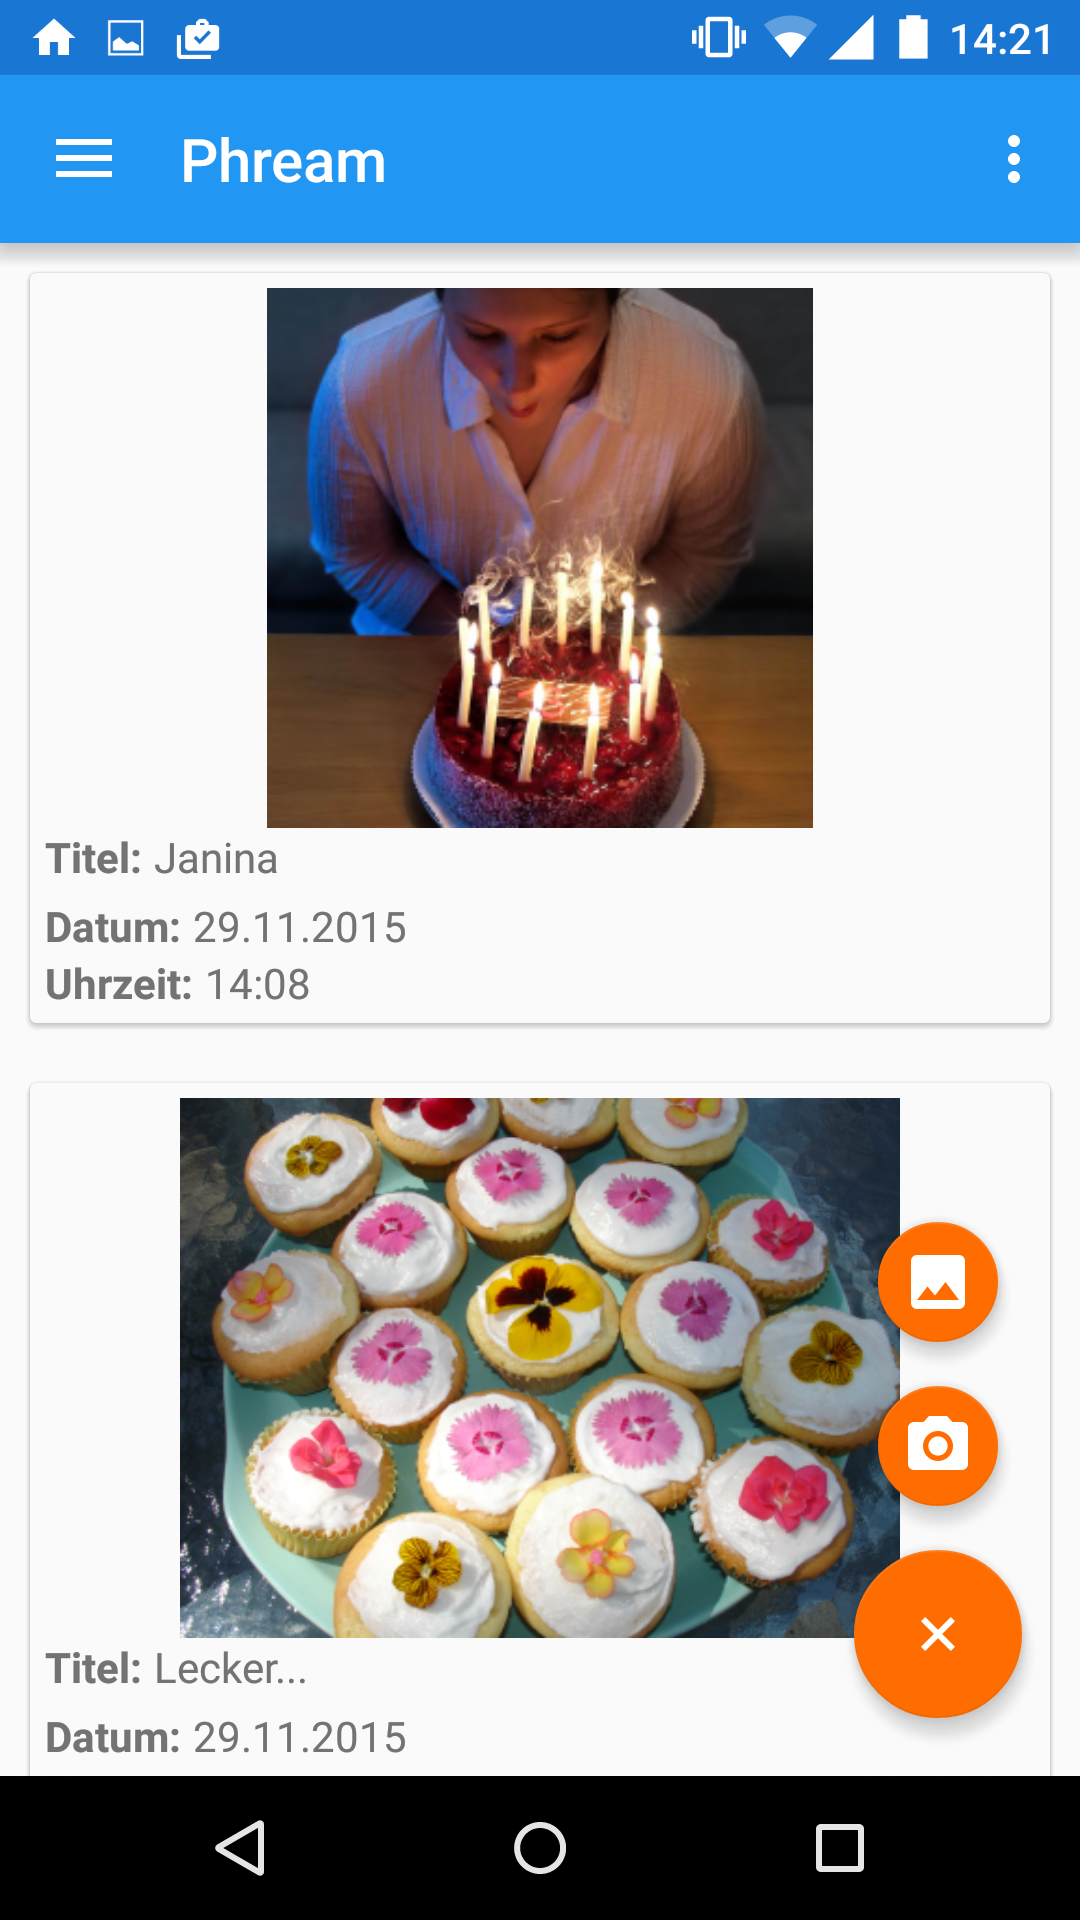
\includegraphics[scale=0.1]{images/screenshots/floatingaction_menu.png}
\caption{Floating Action Menu}
\label{label:floatingaction_menu}
\end{figure}

\subsection{Aufnehmen eines Fotos}
Nach dem Auswählen des Menü Eintrags im Floating Action Menu startet ein Kamera-Intent (Abbildung \ref{label:camera}), über das der Benutzer ein Foto aufnehmen kann und auch alle weiteren Kameraoptionen zur Verfügung hat. Nach dem Bestätigen des aufgenommenen Fotos kann der Benutzer einen Bildtitel (Abbildung \ref{label:camera_imagetitle}) festlegen.
\begin{figure}[H]
\centering
	\begin{minipage}{0.4\textwidth} 
	\centering
	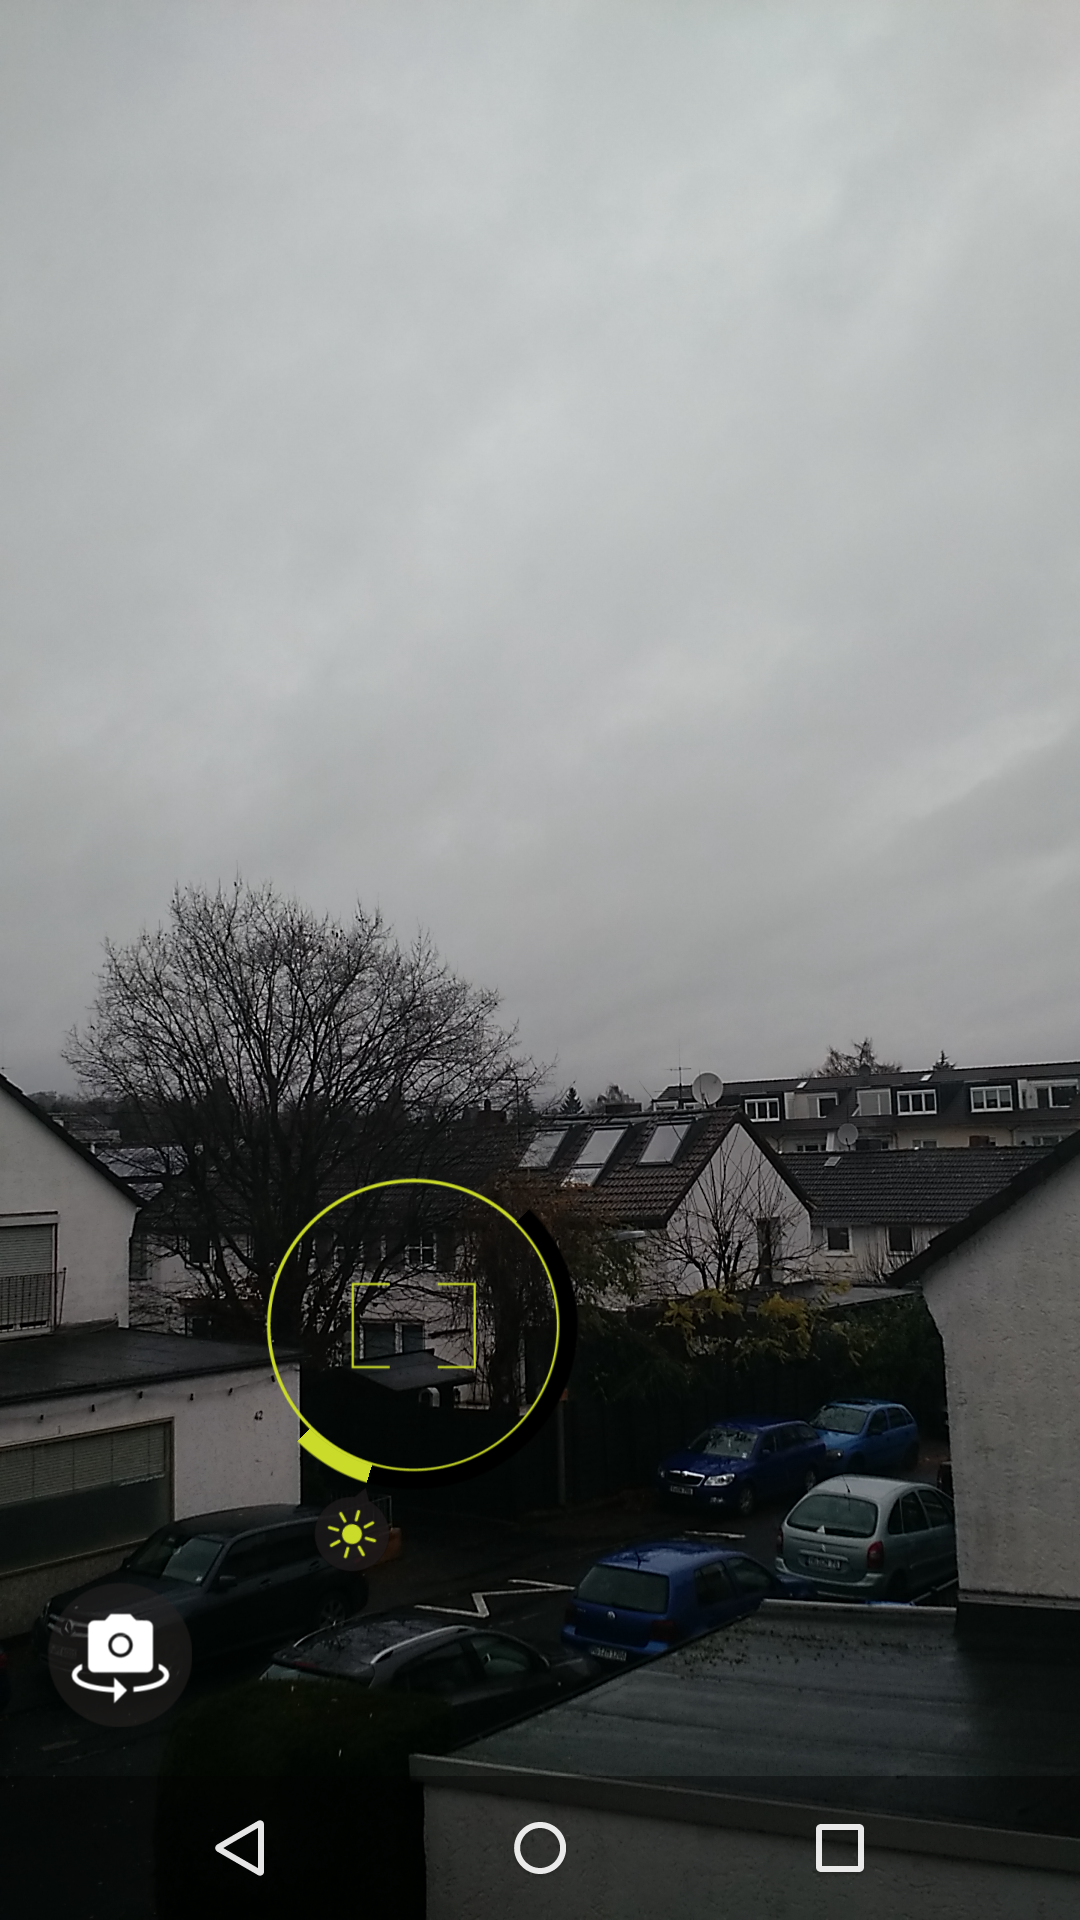
\includegraphics[width=0.6\textwidth]{images/screenshots/camera.png}
	\caption{Kamera-Intent}
	\label{label:camera}
	\end{minipage}
	\hfill
	\begin{minipage}{0.4\textwidth}
	\centering
	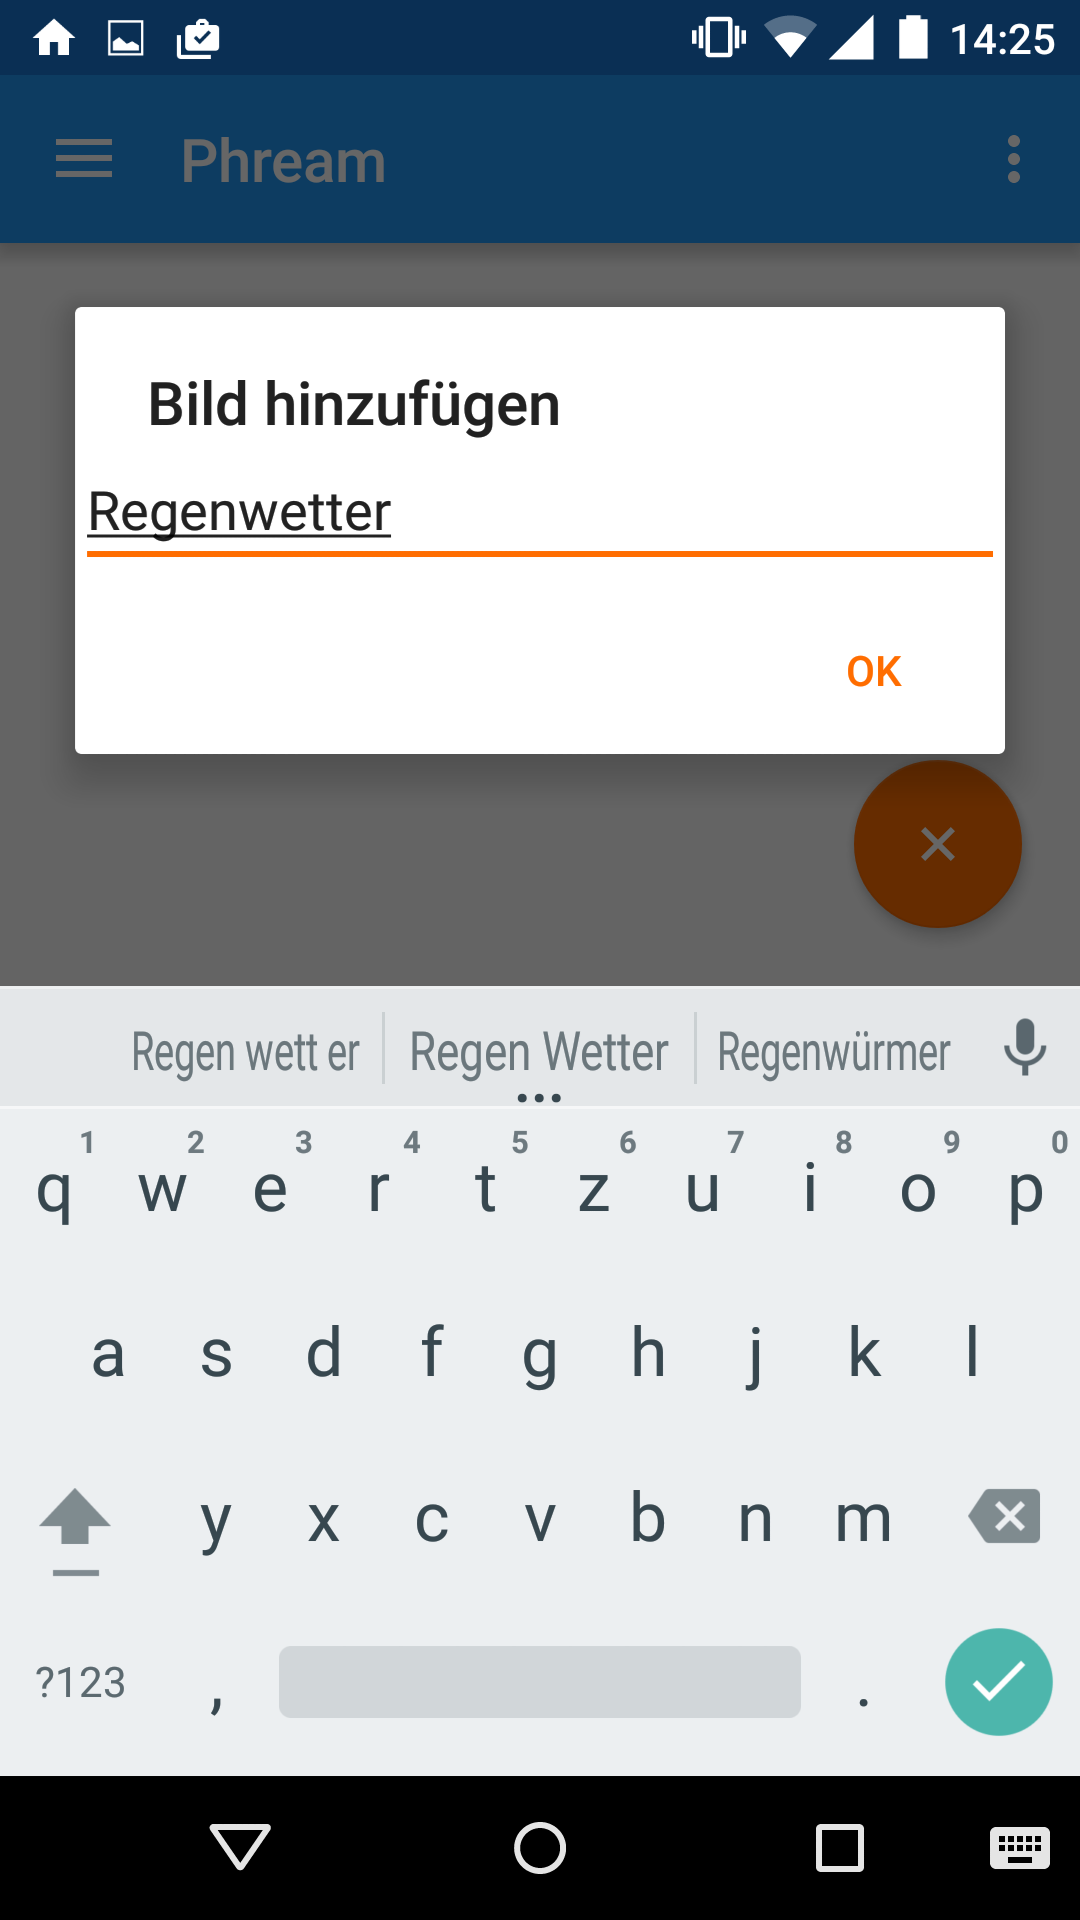
\includegraphics[width=0.6\textwidth]{images/screenshots/camera_imagetitle.png}
	\caption{Bildtitel festlegen}
	\label{label:camera_imagetitle}
	\end{minipage}
\end{figure}

\subsection{Importieren eines Fotos}
Nach dem Auswählen der Importierfunktion im Floating Action Menu startet der Content-Provider (Abbildung \ref{label:content_provider}), der dem Benutzer die Option bietet Dateien (in diesem Fall Bilder) auszuwählen. Dabei beschränkt sich die Dateiauswahl nicht nur auf die eigene Galerie, sondern zeigt auch falls vorhanden, Bilder aus Google Drive oder Dropbox an. Dabei werden die Bilder erst aus der Cloud geladen und dann in die App importiert. Nach dem Importieren des Bildes kann der Benutzer wieder einen Bildtitel festlegen.

\begin{figure}[H]
\centering
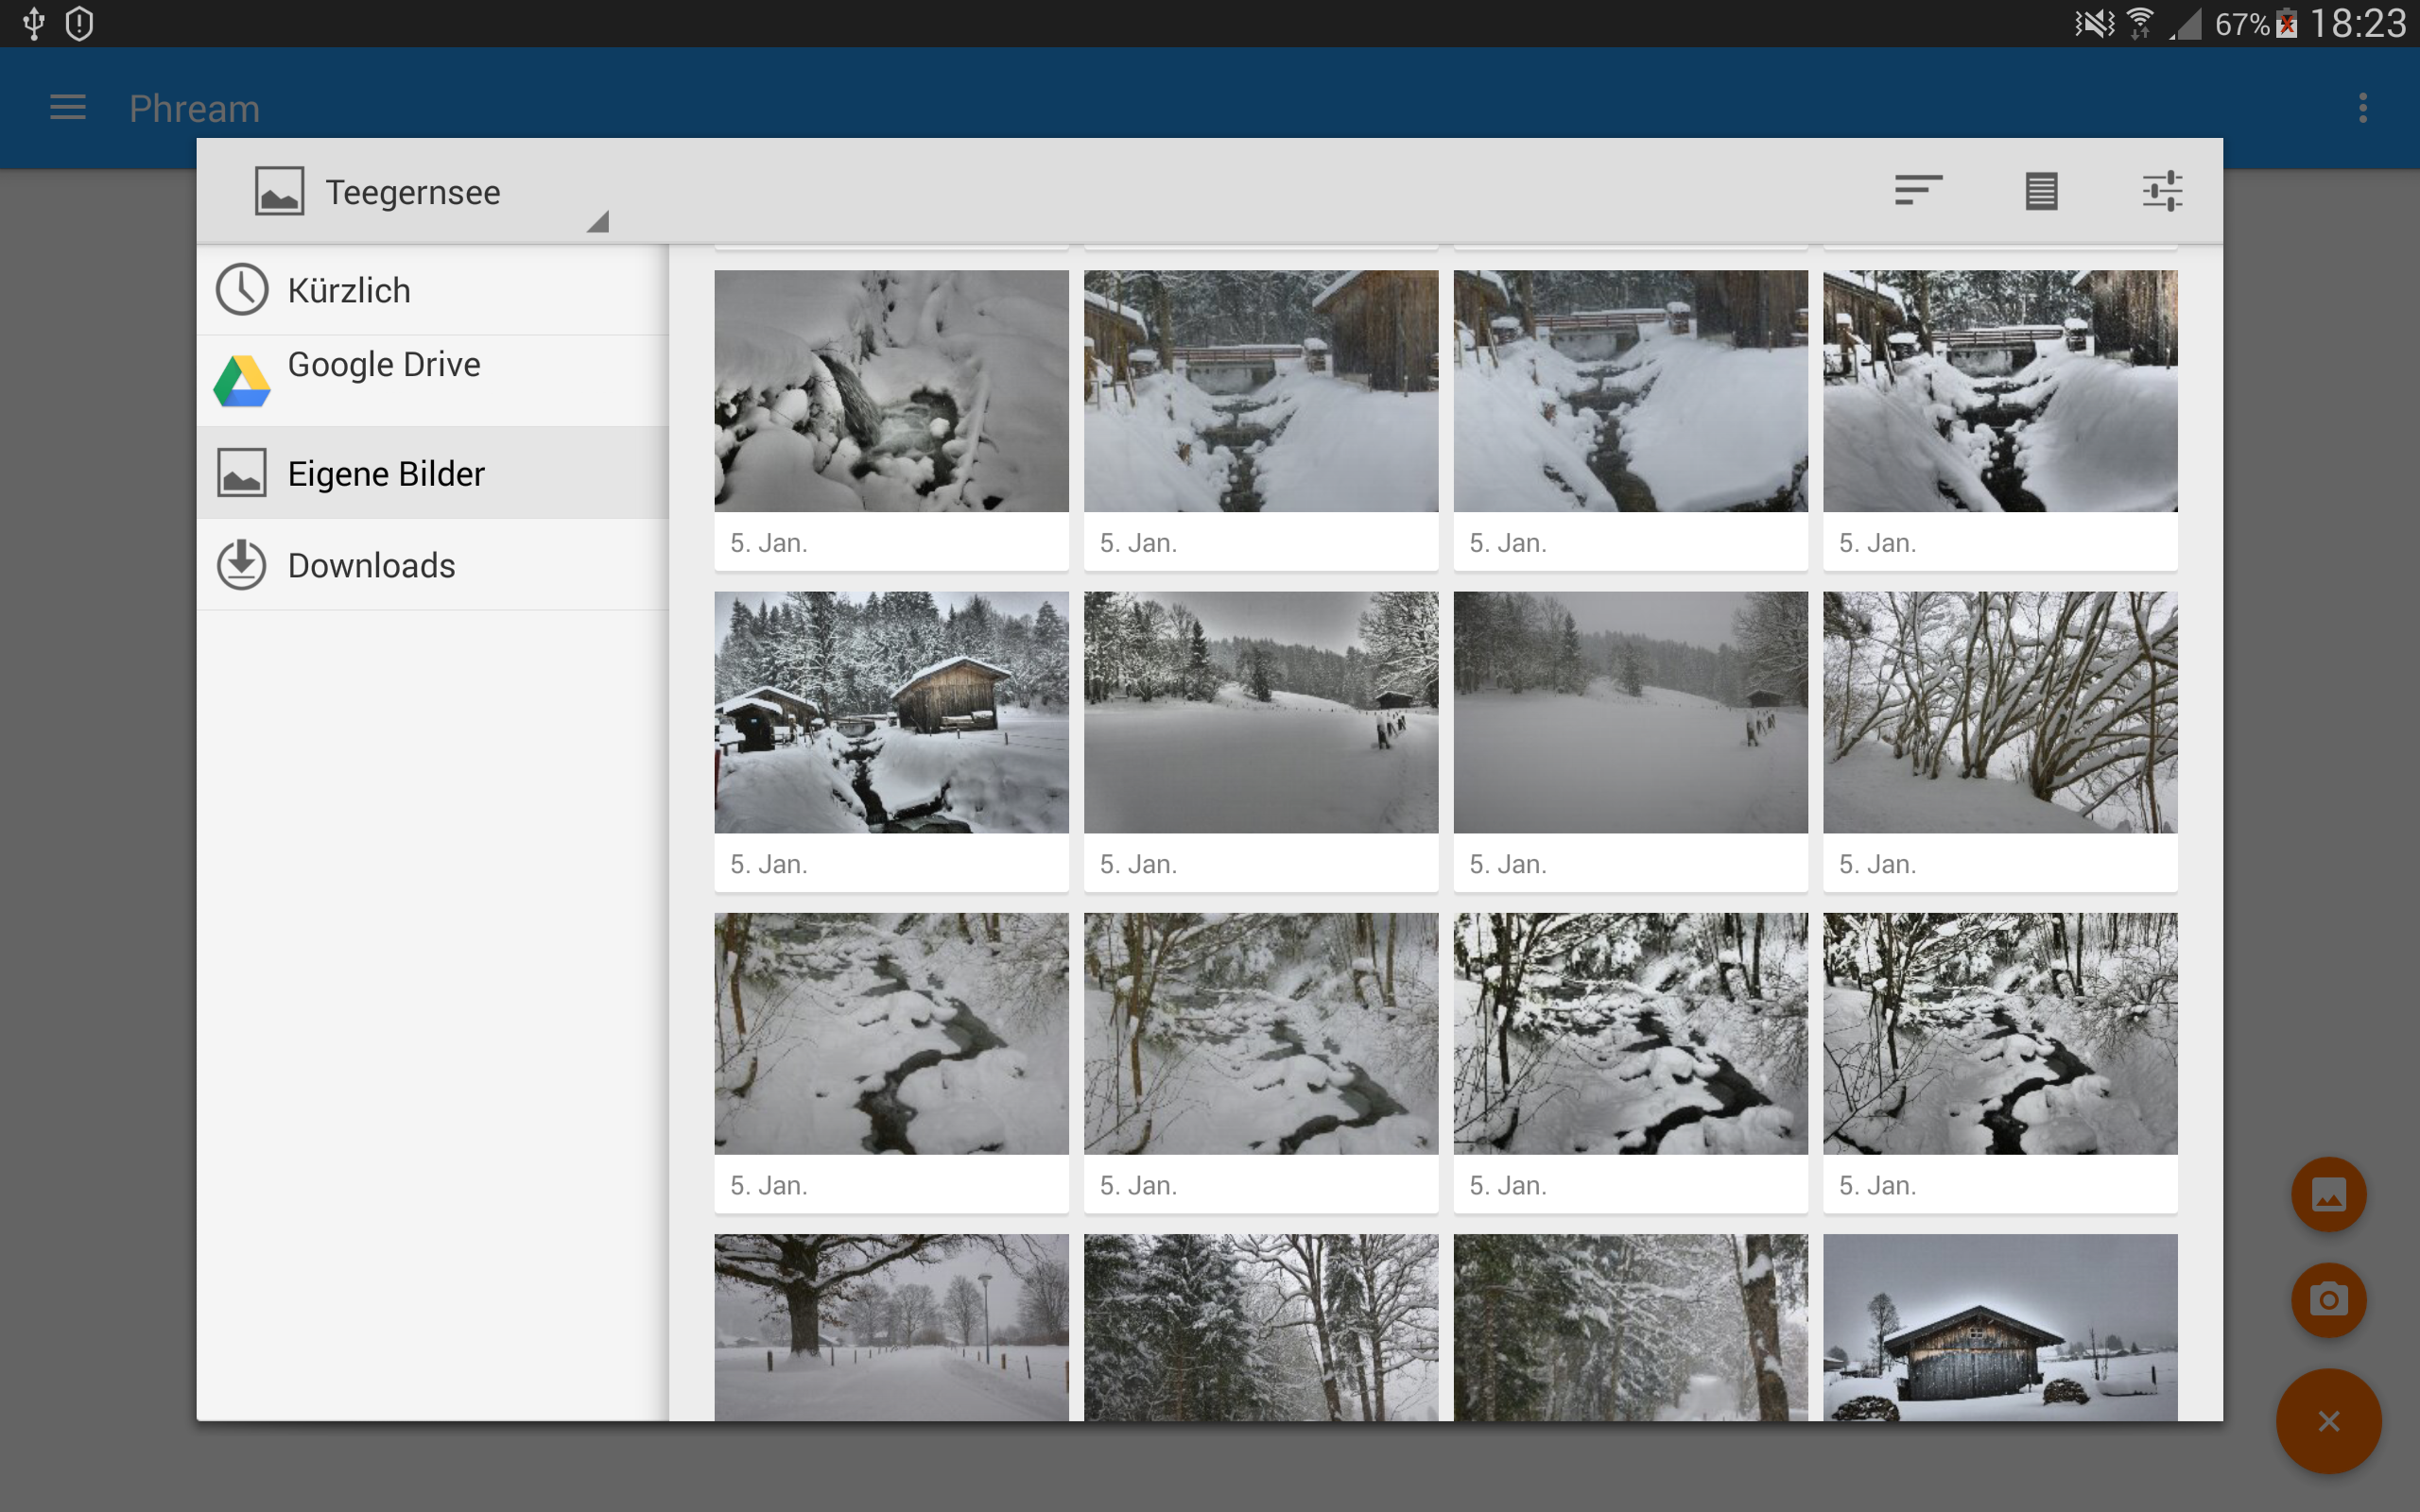
\includegraphics[scale=0.17]{images/screenshots/content_provider.png}
\caption{Content-Provider zum Auswählen eines Bildes}
\label{label:content_provider}
\end{figure}

\section{Verwendete Libraries}
Um verschiedene Benutzeroberflächenelemente auch auf früheren Android Versionen verfügbar zu machen, wurde die AppCompat Support Library\footnote{\url{http://developer.android.com/tools/support-library/features.html}} von Google verwendet. Sie ermöglicht erst in späteren Android Versionen eingefügte Features auch unter älteren Anroid Geräten verfügbar zu machen. Weiterhin wurde zur Gestaltung des Floating Action Menu die AppCompat-Extension-Library\footnote{\url{https://github.com/TR4Android/AppCompat-Extension-Library}} verwendet, um einfach und schnell Floating Action Menu's zu gestalten. Beide Libraries ermöglichen, dass die App ab API-Level 16 verfügbar ist.

Aufgrund eines Bugs in der Standardexportfunktion von Android zum exportieren von Fotos in die Galerie, wurden exportierte Bilder immer am Ende der Galerie mit Datum 1.1.1970 angezeigt. Daher wurde die Klasse \enquote{CapturePhotoUtils}\footnote{\url{https://gist.github.com/samkirton/0242ba81d7ca00b475b9}} von samuelkirton zum Exportieren von Bildern verwendet.